% ============================================================
%  Anexo D: evidencia del banco de pruebas
%  Archivos en Documentation/evidencia_banco y Documentation/figuras
% ============================================================
\section{Evidencia del banco de pruebas}
\label{anx:evidencia}

Este anexo reúne la evidencia de las pruebas realizadas en el banco. Los
archivos se conservan junto con la documentación del proyecto, en la carpeta
\texttt{evidencia\_banco}.

\subsection{Esquemas de conexión}

\begin{figure}[htbp]
    \centering
    \includegraphics[width=0.9\linewidth,height=0.75\textheight,keepaspectratio]%
        {mapa_cableado_esquema.jpg}
    \caption{Esquema de cableado original del dispositivo.}
    \label{fig:mapa_cableado_esquema}
\end{figure}

\begin{figure}[htbp]
    \centering
    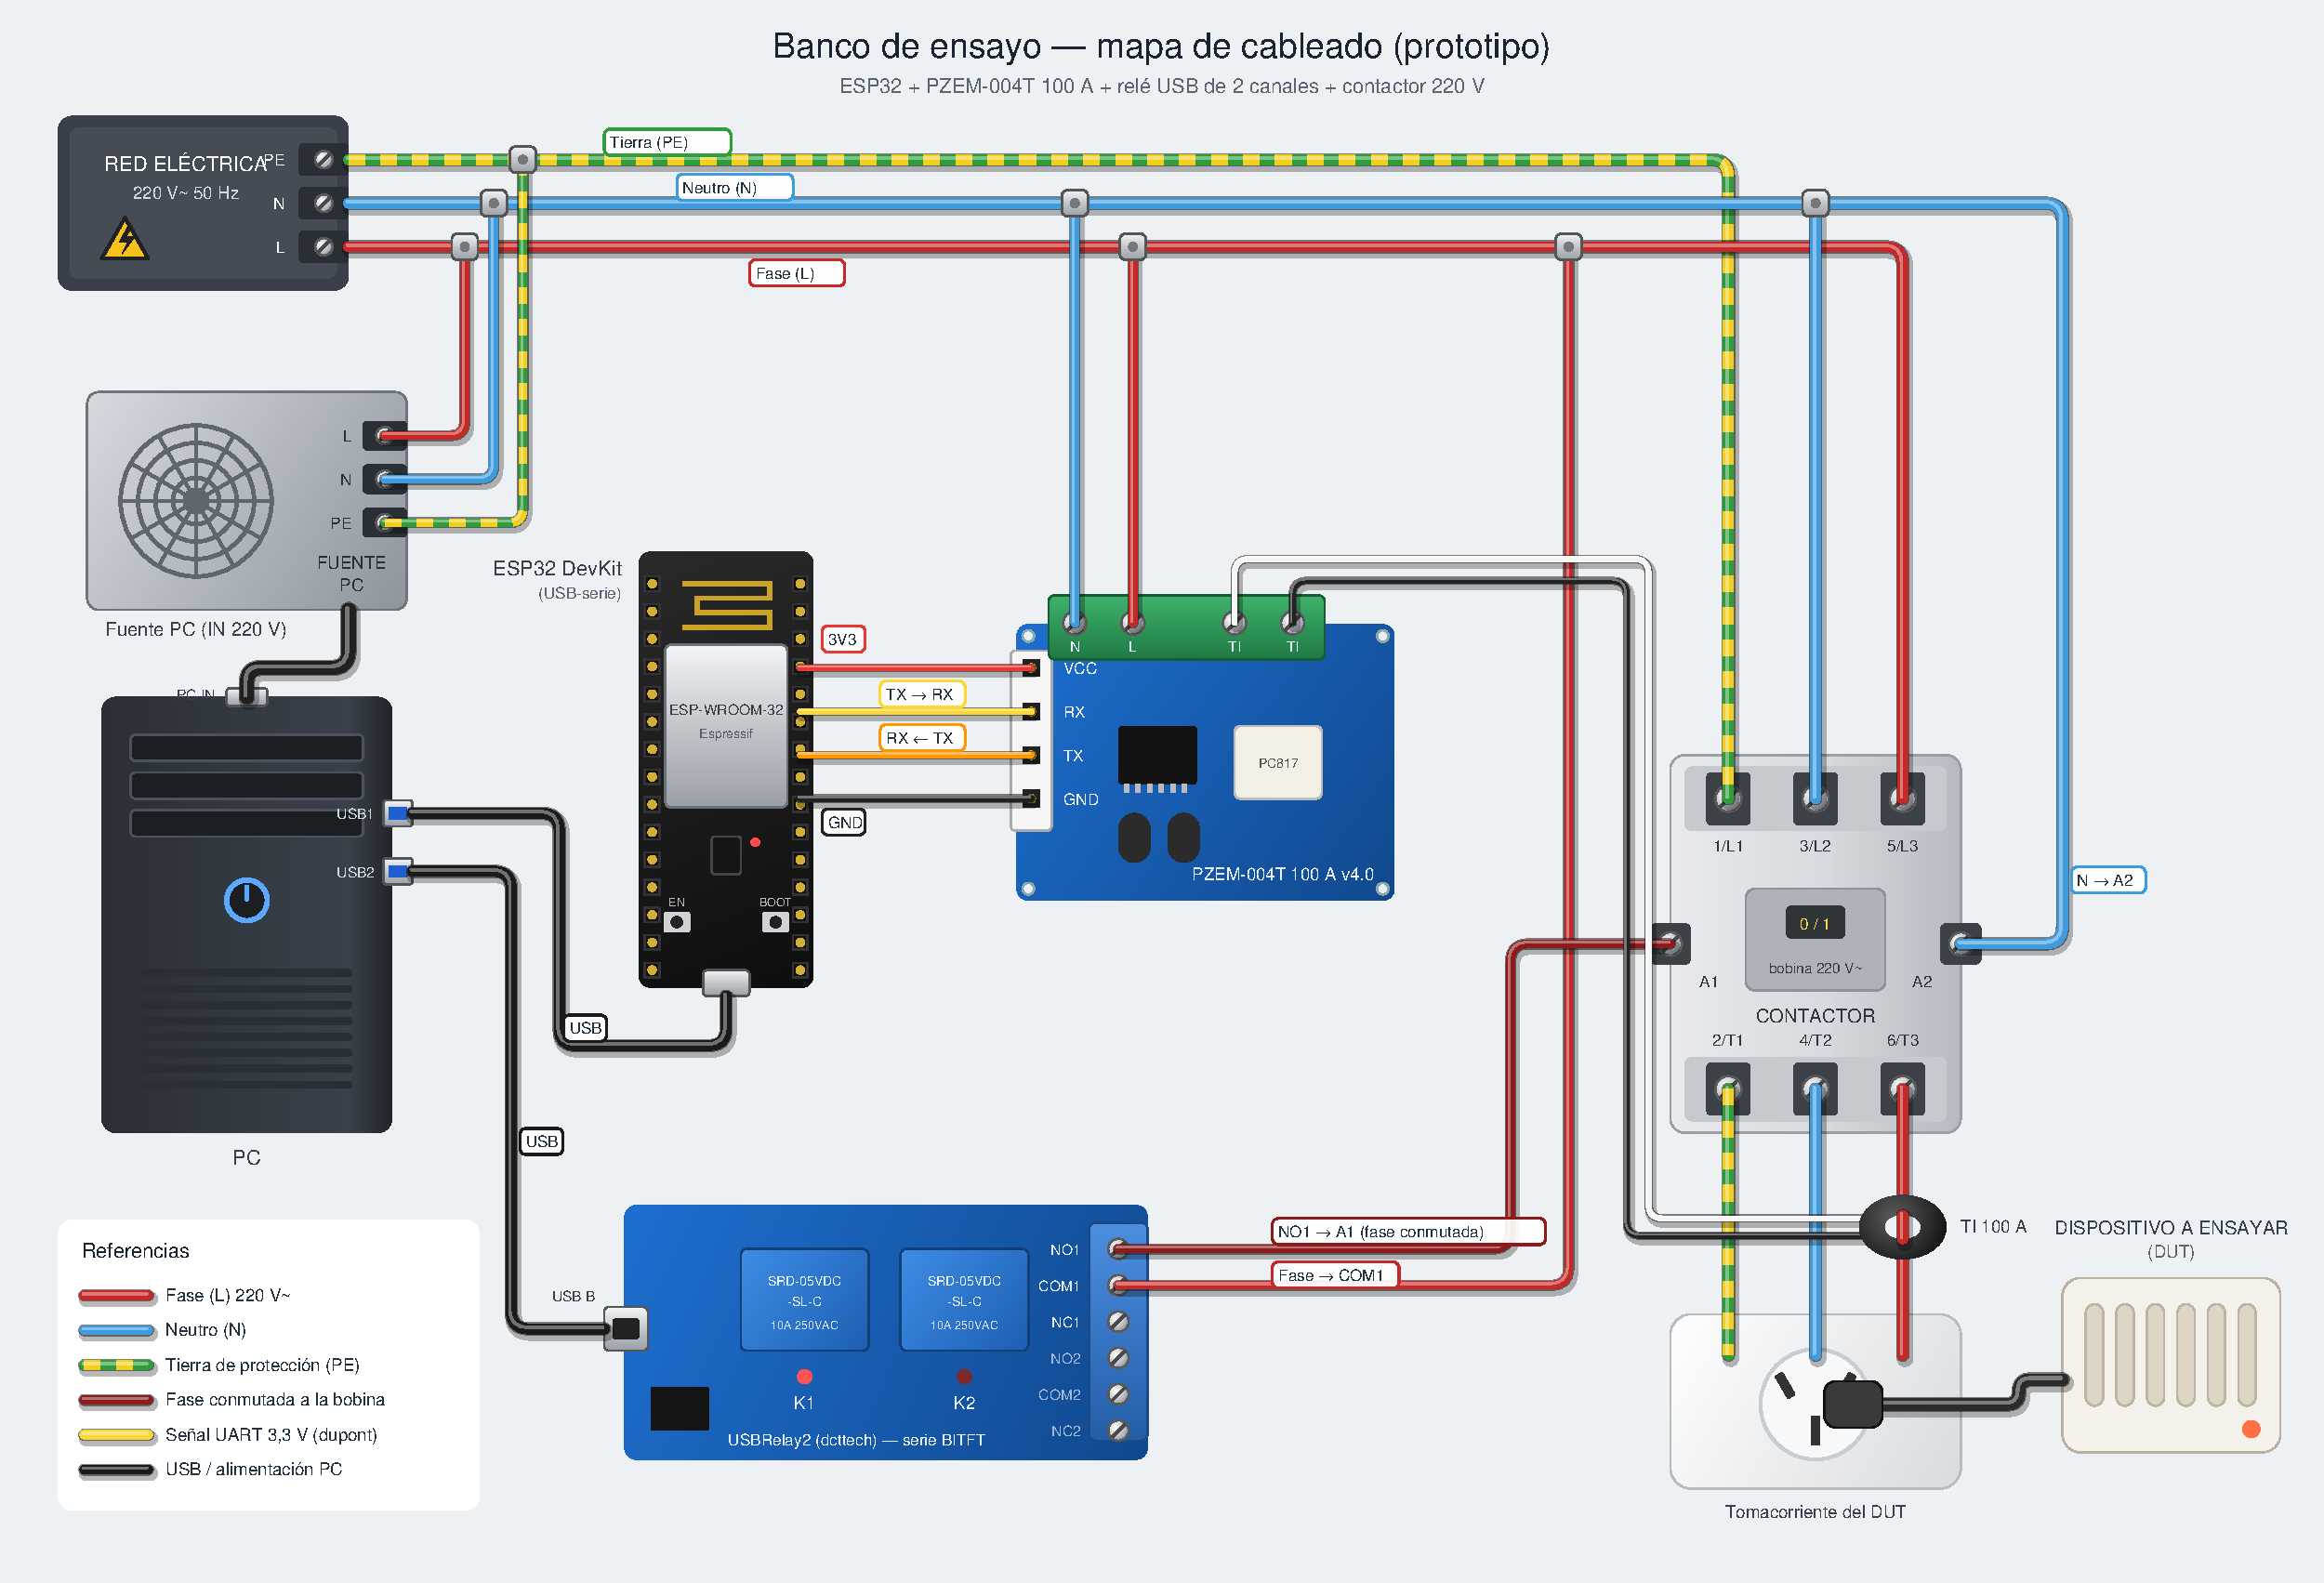
\includegraphics[width=\linewidth]{mapa_cableado.pdf}
    \caption{Versión ilustrada del esquema de cableado.}
    \label{fig:mapa_cableado}
\end{figure}

\subsection{Esquemas de conexión de los ensayos de seguridad}

Las Figuras~\ref{fig:conexion_fuga_activa} a~\ref{fig:conexion_pat} muestran el
\textbf{diseño propuesto} de conexión de los ensayos de seguridad, elaborado por
la autora a partir del equipo completo de SYGlab y de los requisitos de la norma.
No es hardware implementado en el prototipo propio: cada esquema indica la
secuencia que ejecuta el software y, en un recuadro, los puntos que quedan por
definir para construirlo (por ejemplo, la resolución del medidor para
\SI{0,75}{\milli\ampere} o la medición de la caída de tensión en puesta a
tierra).

\begin{figure}[htbp]
    \centering
    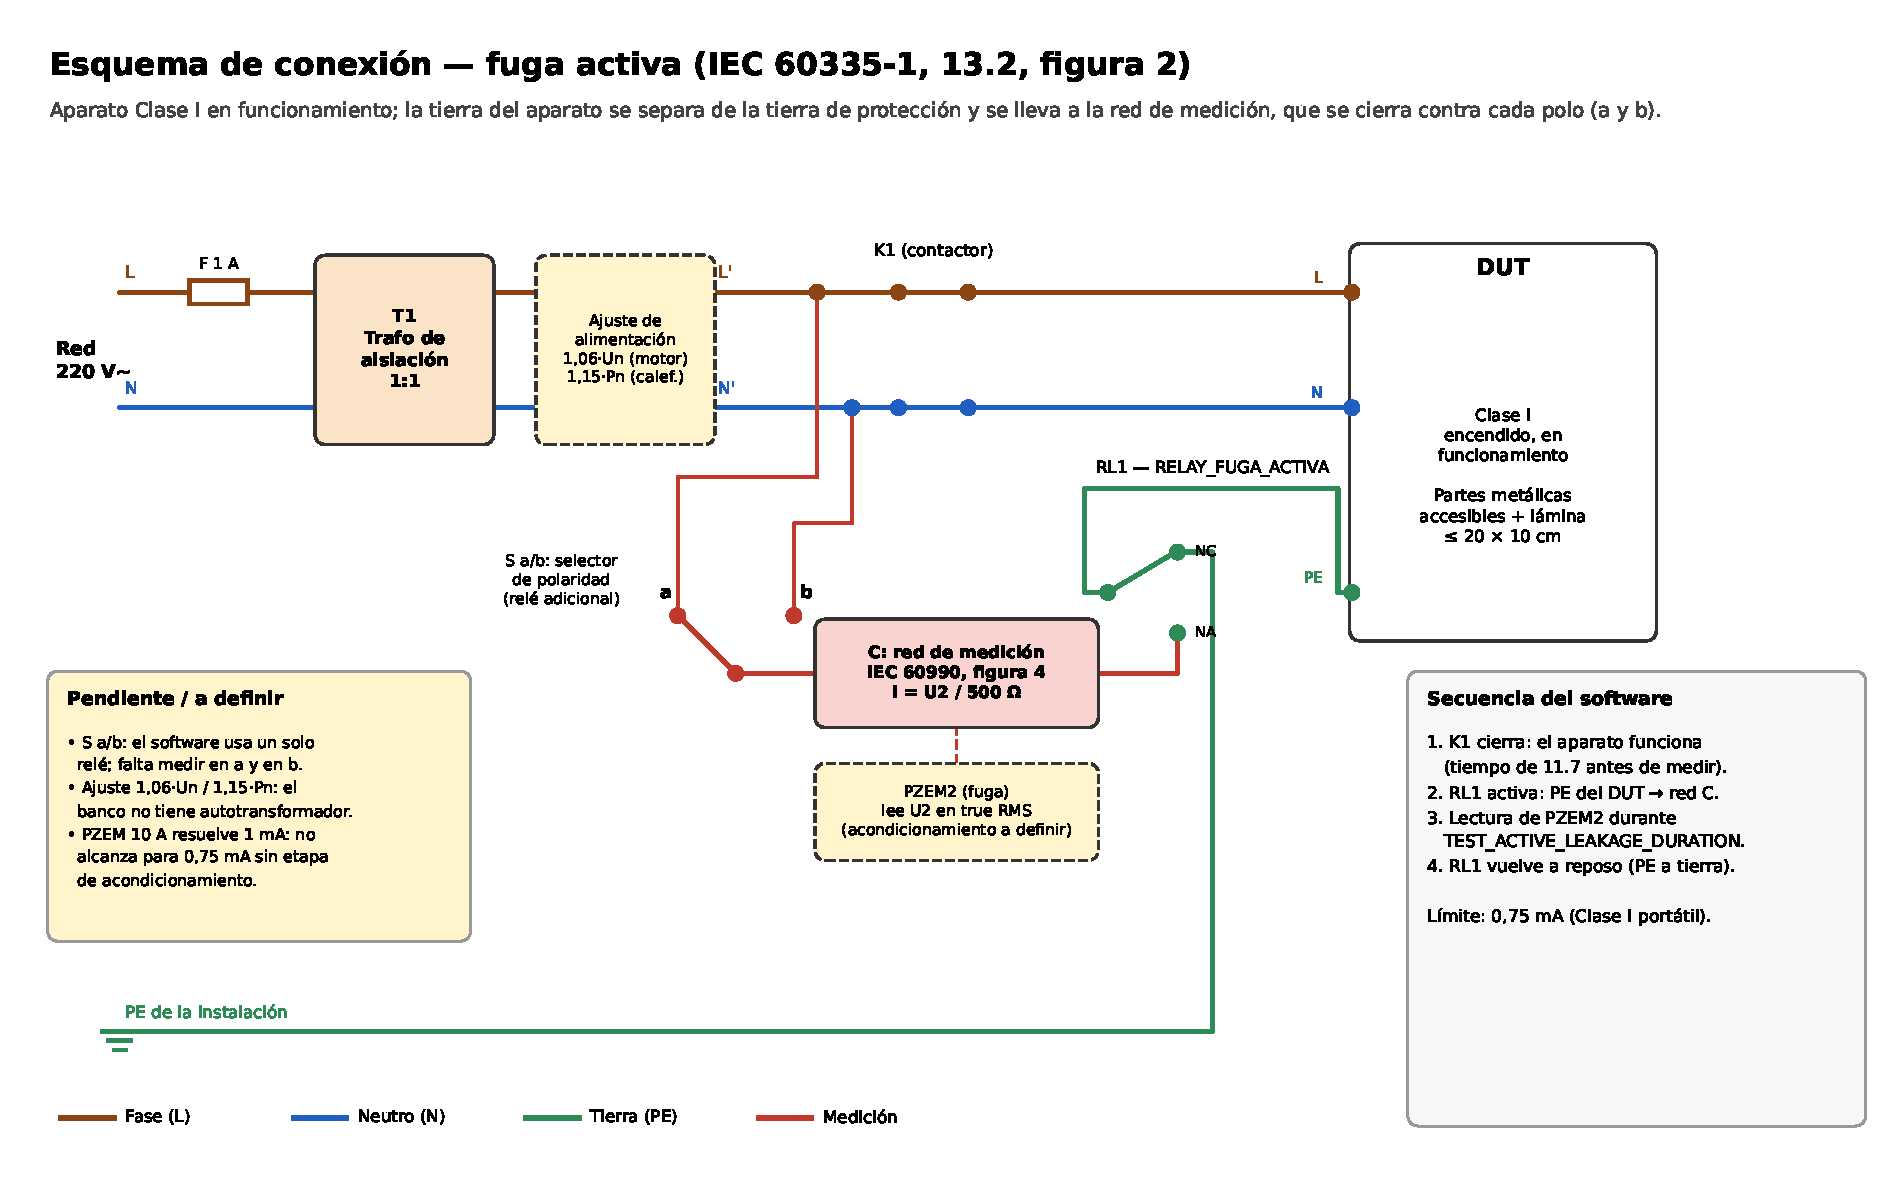
\includegraphics[width=\linewidth]{conexion_fuga_activa.pdf}
    \caption{Esquema de conexión del ensayo de fuga activa (IEC~60335-1, 13.2).}
    \label{fig:conexion_fuga_activa}
\end{figure}

\begin{figure}[htbp]
    \centering
    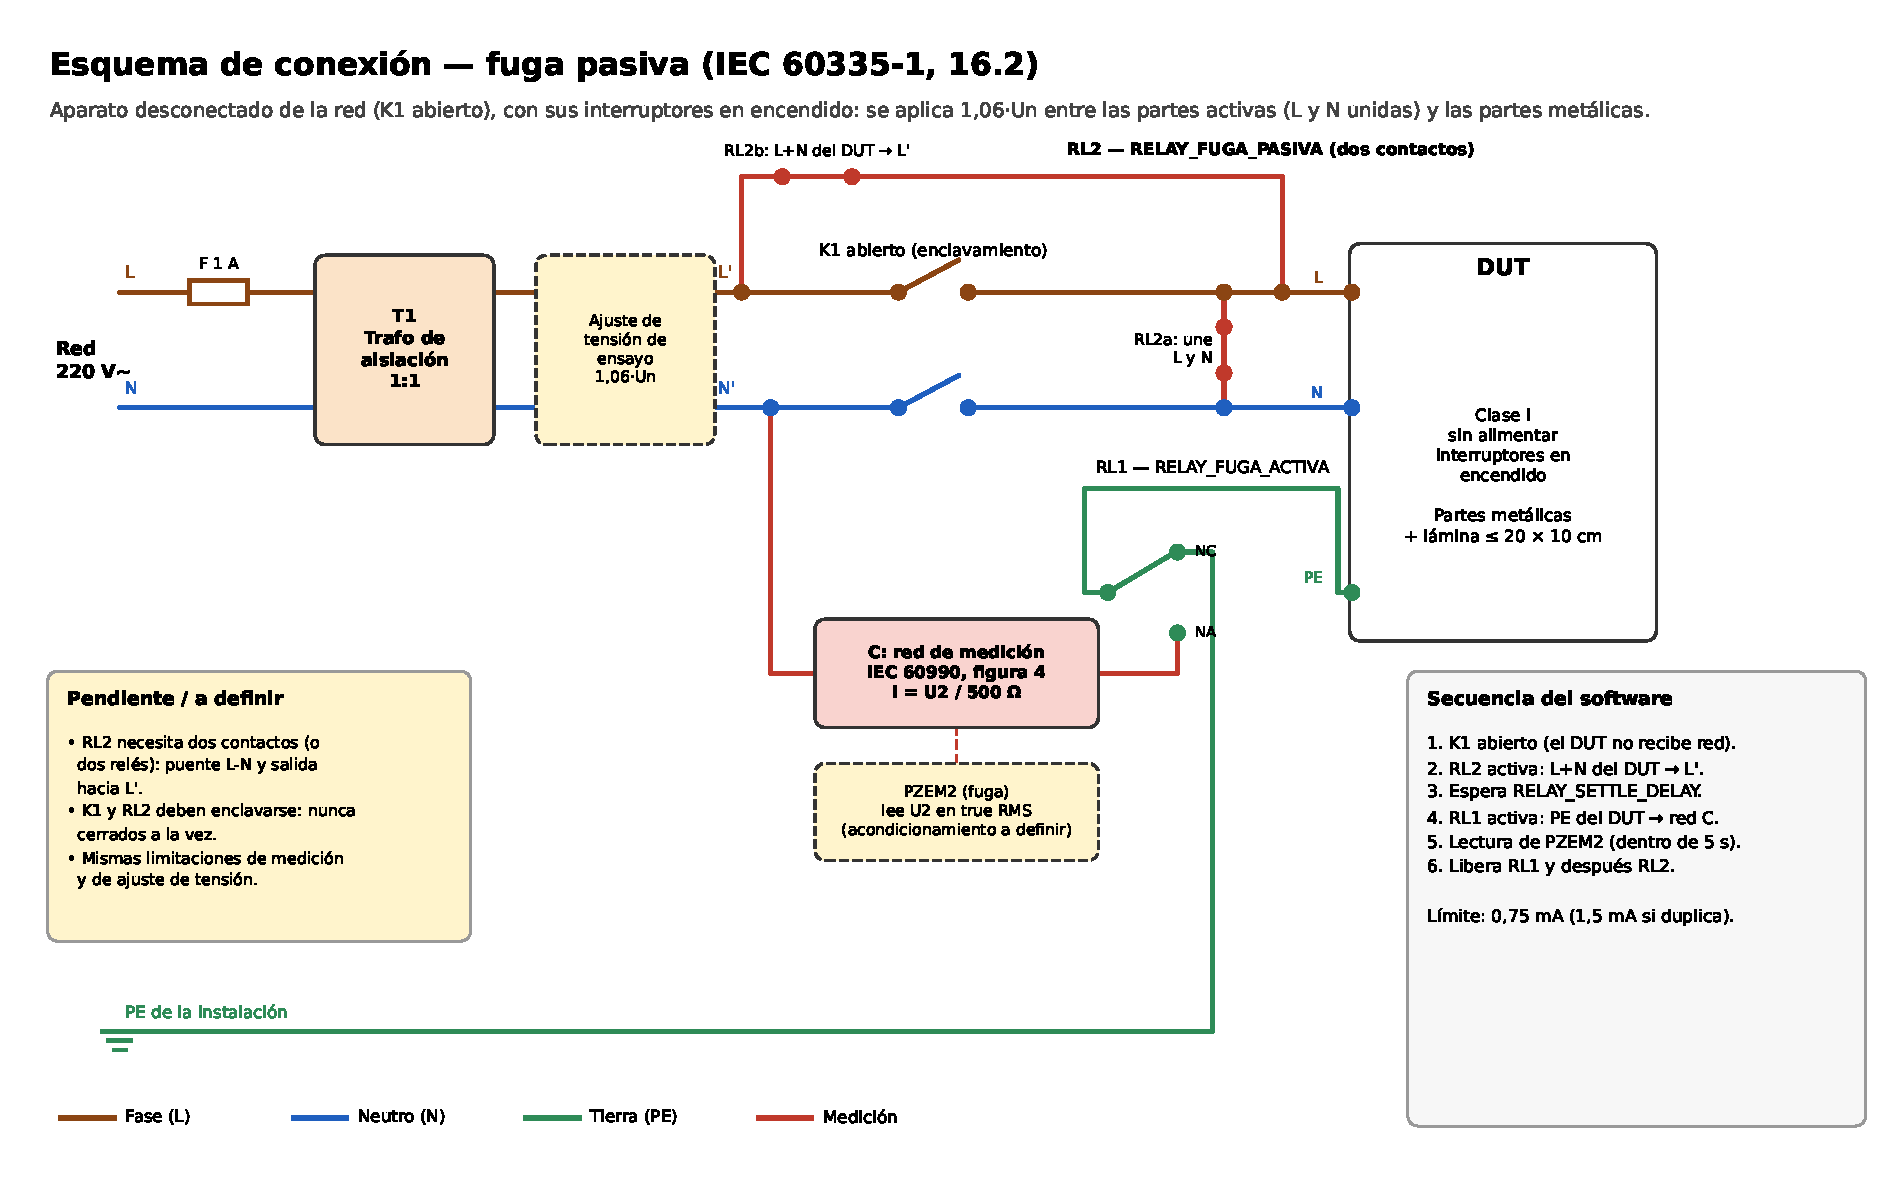
\includegraphics[width=\linewidth]{conexion_fuga_pasiva.pdf}
    \caption{Esquema de conexión del ensayo de fuga pasiva (IEC~60335-1, 16.2).}
    \label{fig:conexion_fuga_pasiva}
\end{figure}

\begin{figure}[htbp]
    \centering
    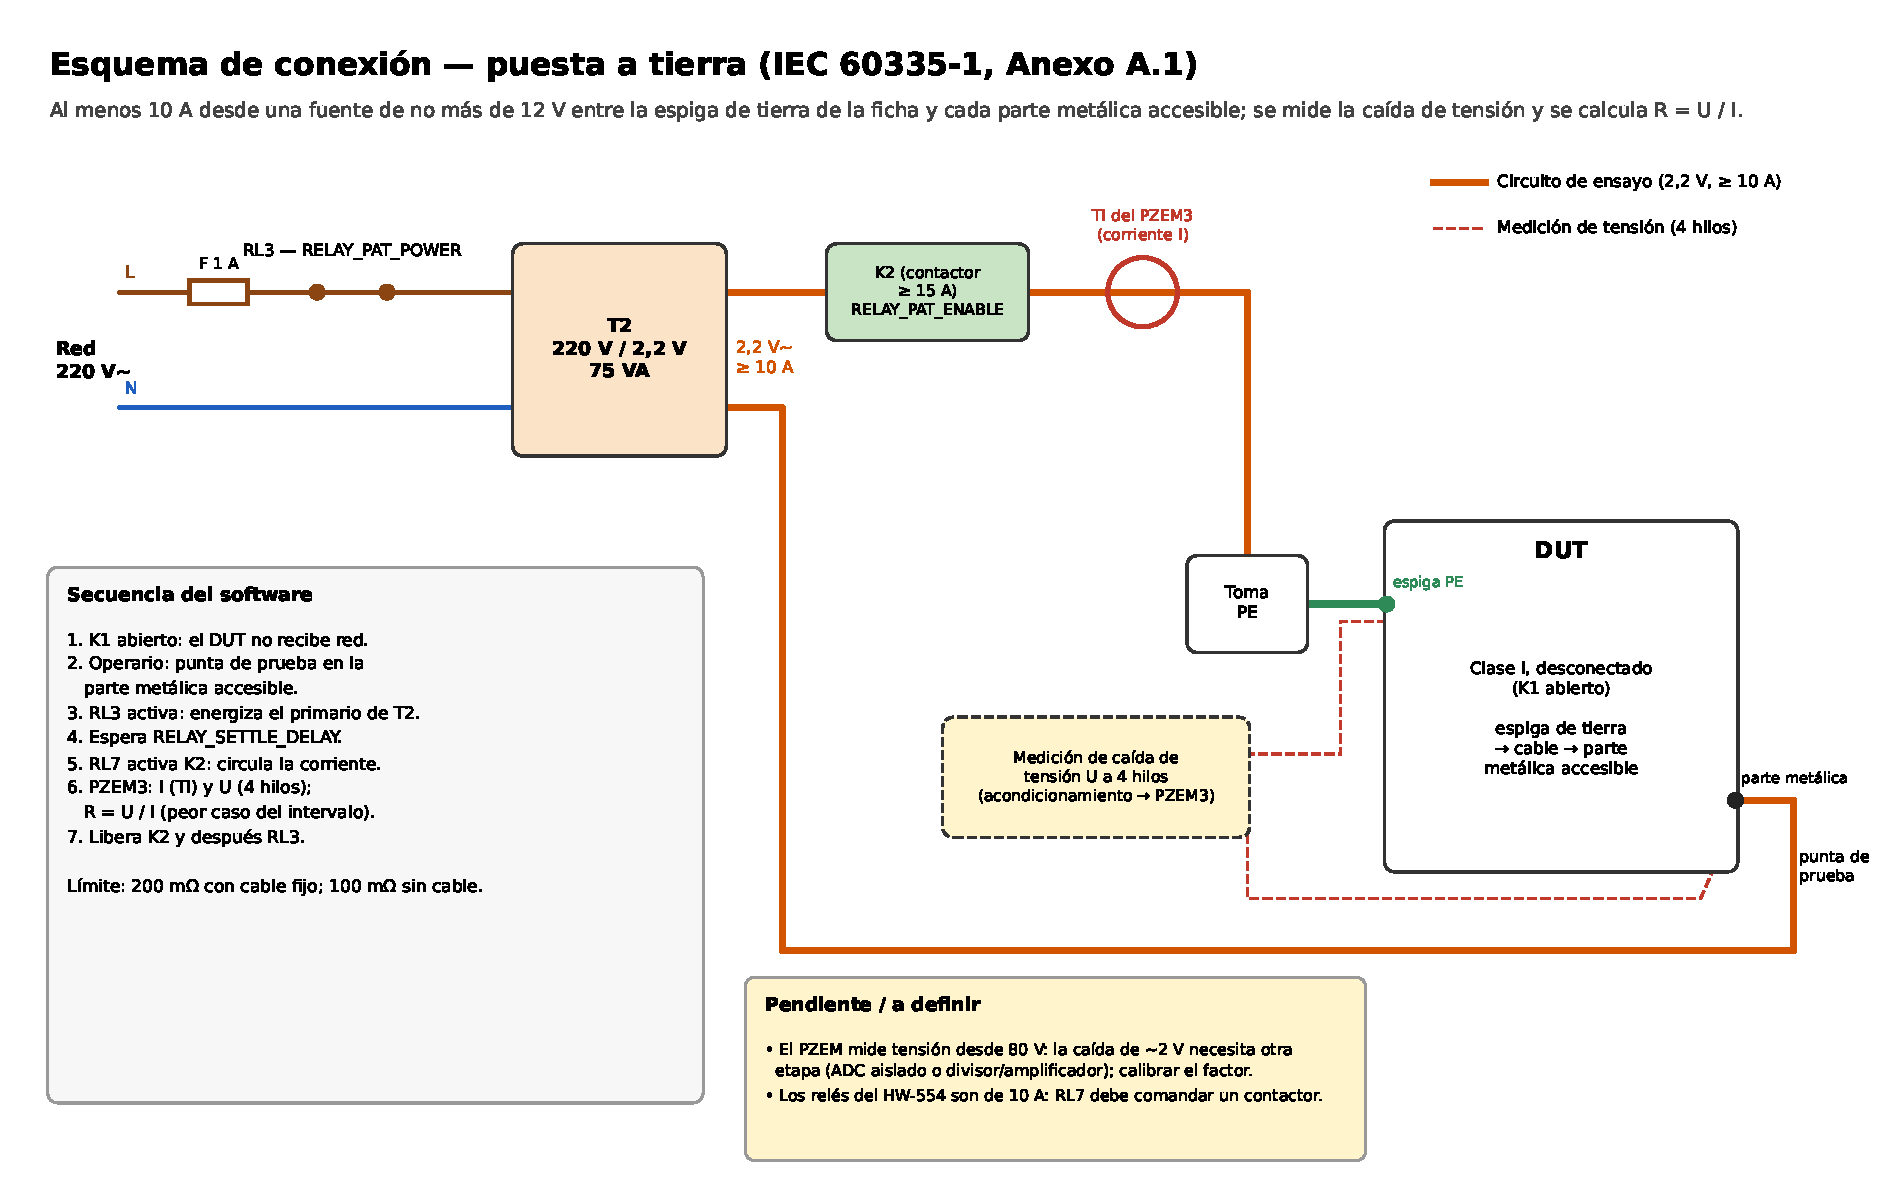
\includegraphics[width=\linewidth]{conexion_pat.pdf}
    \caption{Esquema de conexión del ensayo de puesta a tierra (IEC~60335-1,
             Anexo~A.1).}
    \label{fig:conexion_pat}
\end{figure}

\subsection{Fotografías}

La Figura~\ref{fig:equipo_completo} muestra el equipo completo de referencia
armado, con los contactores de cada ensayo (consumo, puesta a tierra y tensión
resistida de \SI{1}{\kilo\volt} y \SI{2,5}{\kilo\volt}), los transformadores de
ensayo, el módulo de relés y las borneras. La Figura~\ref{fig:banco_prototipo}
muestra el primer prototipo propio durante el ensayo de consumo del soldador.

\begin{figure}[htbp]
    \centering
    \begin{subfigure}[b]{0.66\linewidth}
        \centering
        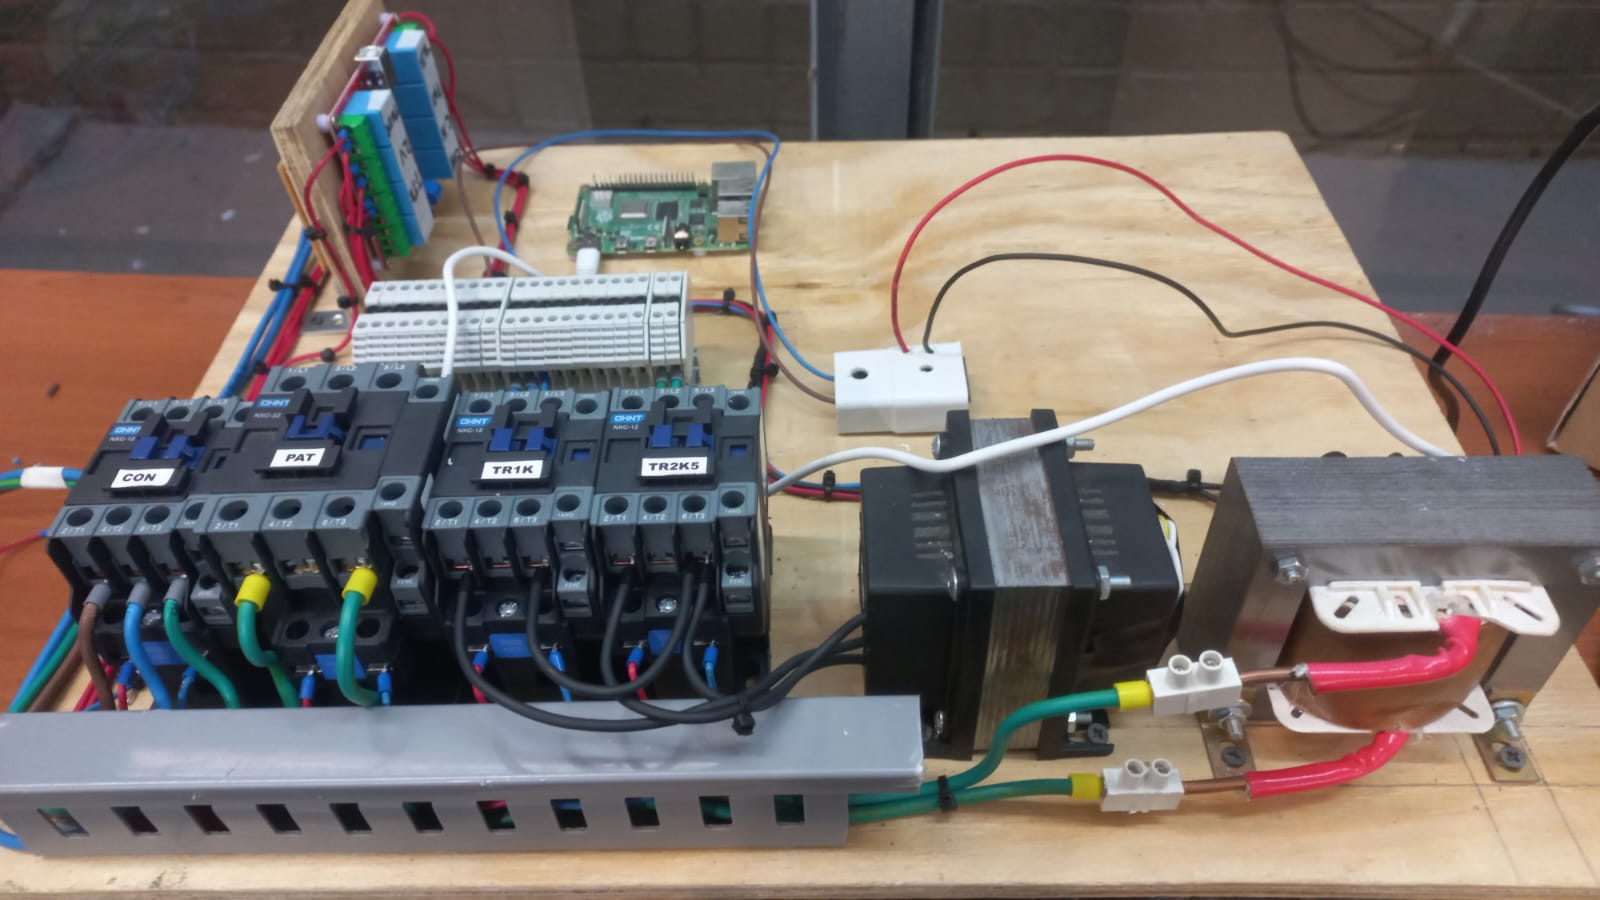
\includegraphics[height=5.8cm]{equipo_completo_general.jpg}
        \caption{Vista general.}
    \end{subfigure}\hfill
    \begin{subfigure}[b]{0.30\linewidth}
        \centering
        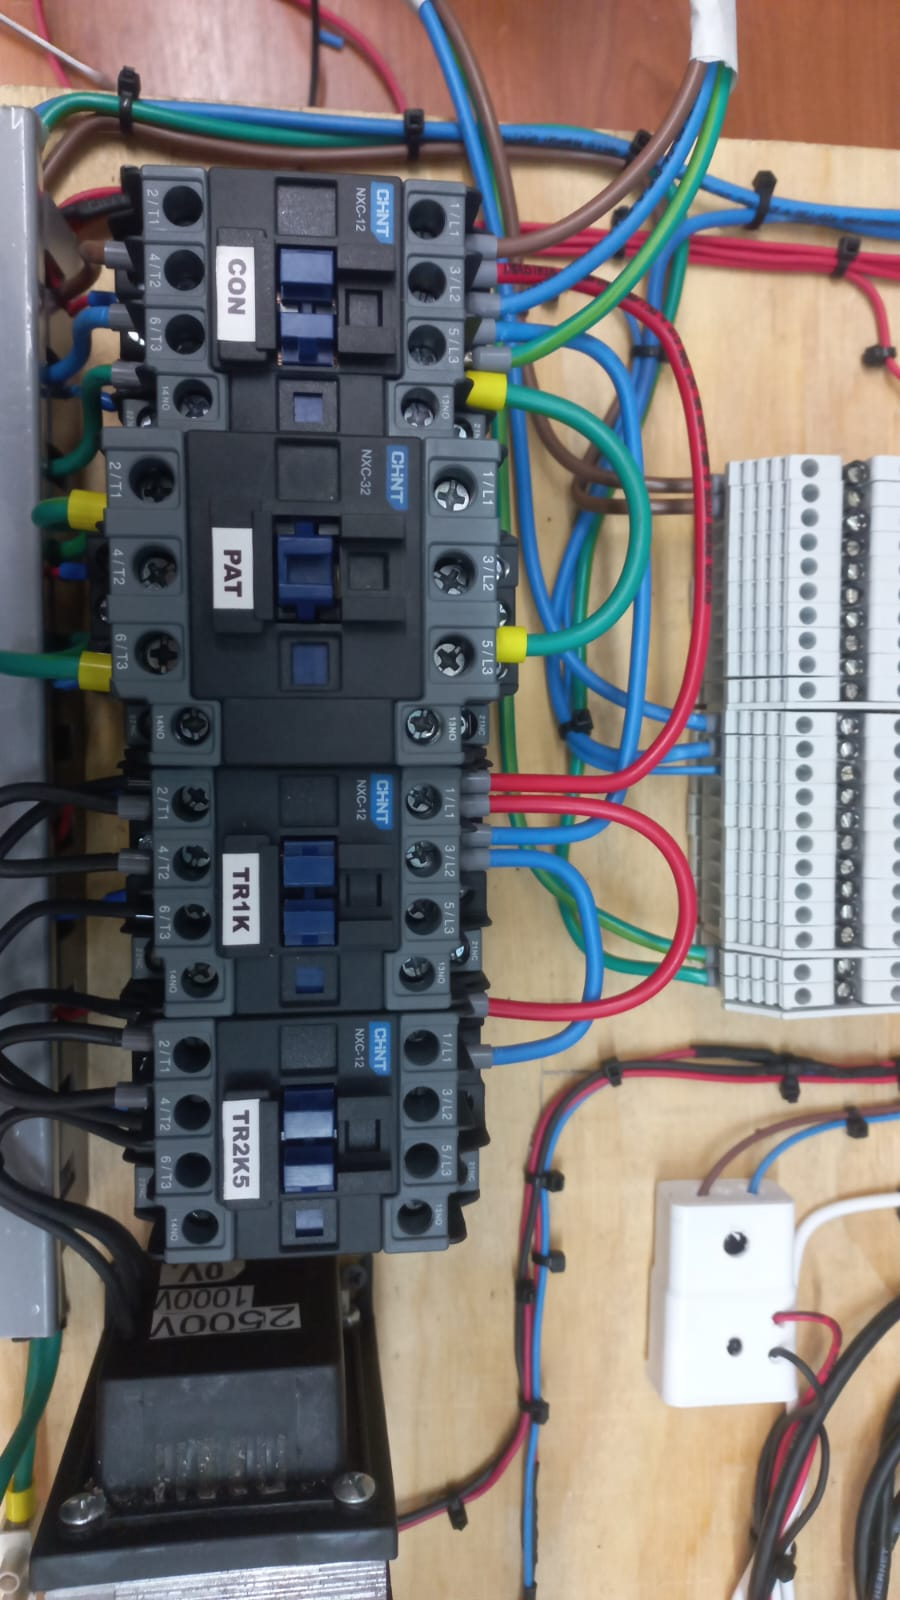
\includegraphics[height=6cm]{equipo_completo_contactores.jpg}
        \caption{Contactores de cada ensayo.}
    \end{subfigure}
    \caption{Equipo completo de referencia armado.}
    \label{fig:equipo_completo}
\end{figure}

\begin{figure}[htbp]
    \centering
    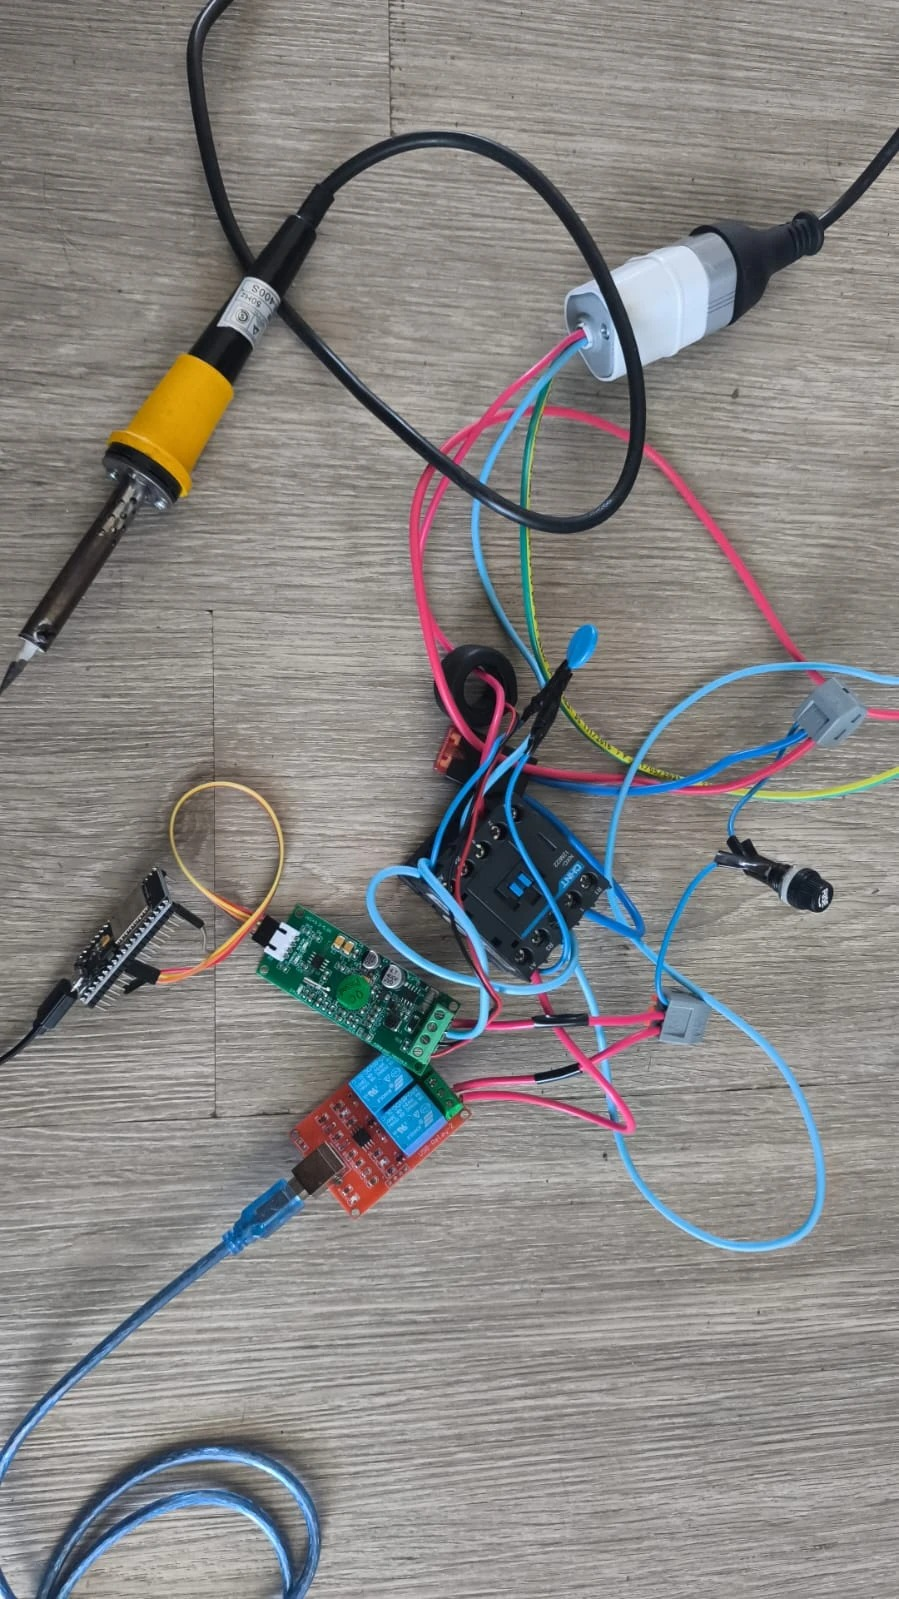
\includegraphics[height=0.6\textheight,keepaspectratio]{banco_prototipo_soldador.jpg}
    \caption{Primer prototipo propio (ESP32, PZEM-004T, placa de relés USB y
             contactor) durante el ensayo de consumo del soldador.}
    \label{fig:banco_prototipo}
\end{figure}

\subsection{Registro de hallazgos}

La Tabla~\ref{tab:hallazgos} resume los hallazgos principales y su resolución.

\begin{longtable}{@{} p{4.2cm} p{5.3cm} p{5.3cm} @{}}
\caption{Hallazgos principales y su resolución}\label{tab:hallazgos}\\
\toprule
\textbf{Hallazgo} & \textbf{Causa} & \textbf{Resolución} \\
\midrule
\endfirsthead
\toprule
\textbf{Hallazgo} & \textbf{Causa} & \textbf{Resolución} \\
\midrule
\endhead
\multicolumn{3}{@{}l}{\textit{Normativos}} \\
Rigidez evaluada solo por tensión
  & Se tomó la corriente de la fuente como límite de aprobación
  & Criterio del Anexo~A.2: corriente $\leq$ \SI{5}{\milli\ampere} con la
    tensión de ensayo aplicada \\
Fuga pasiva con límite fijo de \SI{1500}{\micro\ampere}
  & Se usaba siempre el límite duplicado
  & \SI{750}{\micro\ampere}; \SI{1500}{\micro\ampere} solo con condición de
    duplicación (16.2) \\
Puesta a tierra con límite único
  & Sin distinguir cable fijo ni controlar la corriente
  & \SI{200}{\milli\ohm} o \SI{100}{\milli\ohm} con corriente
    $\geq$ \SI{10}{\ampere} (A.1) \\
Consumo con porcentajes fijos
  & Tolerancia única para todos los aparatos
  & Tablas~1 y~2 según tipo y potencia nominal \\
\midrule
\multicolumn{3}{@{}l}{\textit{Hardware}} \\
ESP32 no detectado
  & Cable USB solo de carga; faltaba el controlador CP210x
  & Cambio de cable e instalación del controlador \\
ESP32 no respondía
  & Firmware de fábrica (comandos AT)
  & Firmware propio \\
Bucle de arranque del ESP32
  & Medidor en el puerto del USB y alimentado con \SI{5}{\volt}
  & Medidor en GPIO16/17 alimentado con \SI{3,3}{\volt} \\
Bornes del medidor sin identificar
  & Bornera sin serigrafía
  & Identificación por resistencia con multímetro \\
Desconexión de la placa de relés
  & Interferencia al abrir el contactor con carga con motor
  & Software tolerante con falla segura y varistor en la bobina (mitigado) \\
Medidor sin resolución para fuga
  & Umbral de arranque de unos \SI{20}{\milli\ampere}
  & Requiere versión de \SI{10}{\ampere} y red IEC~60990 (pendiente) \\
\midrule
\multicolumn{3}{@{}l}{\textit{Software}} \\
Interfaz sin lógica
  & Ventana principal en estado de esqueleto
  & Integración de las ocho pestañas \\
Integración continua sin pruebas
  & Configuración sin las dependencias de desarrollo
  & Flujo corregido; 62 errores de estilo resueltos \\
Correcciones de calibración sin efecto
  & Nunca se aplicaban a las lecturas
  & Aplicadas a todas las lecturas \\
Consumo subestimado \SI{27}{\percent}
  & Lecturas del transitorio de cierre en el promedio
  & Descarte de lecturas de estabilización \\
Credenciales de fábrica en la API
  & Contraseña en texto plano
  & Hash PBKDF2-SHA256 y rechazo de credenciales de fábrica \\
Fuga sin medidor: NO EJECUTADO
  & Lectura fallida sin veredicto
  & Lectura fallida = FALLA en ensayos de seguridad \\
\bottomrule
\end{longtable}

\subsection{Datos y scripts}

\begin{itemize}
    \item Base de datos de la prueba de punta a punta (16 ensayos y 10 muestras de perfil de consumo).
    \item Exportación a Excel generada por la aplicación.
    \item Cuaderno de comandos con las lecturas directas del ventilador y del
          soldador.
    \item Scripts de prueba que operan la aplicación real con el
          hardware real.
\end{itemize}
